\documentclass[11pt]{article}
\usepackage[a4paper,margin=0.85in]{geometry}
\usepackage{amsmath,amssymb}
\usepackage{graphicx}
\usepackage{booktabs}
\usepackage{longtable}
\usepackage{array}
\usepackage{float}
\usepackage{xcolor}
\usepackage{hyperref}
\usepackage{listings}
\usepackage{fancyhdr}
\usepackage{caption}
\usepackage{microtype}
\hypersetup{colorlinks=true,linkcolor=blue,urlcolor=blue}
\pagestyle{fancy}
\fancyhf{}
\lhead{Crypto regime-change detection}
\rhead{L\'opez de Prado structural-break methods}
\cfoot{\thepage}
\setlength{\headheight}{14pt}
\setlength{\parskip}{0.55em}
\setlength{\parindent}{0pt}
\definecolor{boxgray}{RGB}{245,245,245}
\lstset{basicstyle=\ttfamily\footnotesize,breaklines=true,backgroundcolor=\color{boxgray},frame=single,columns=fullflexible}

\title{\Huge Detecting Structural Breaks in Crypto Markets\\[0.25em]
\Large A beginner-friendly empirical report inspired by structural-break methods in \emph{Advances in Financial Machine Learning}}
\author{Prepared from Binance daily OHLC market data}
\date{Generated on %%GENERATED_DATE%%}

\begin{document}
\maketitle

\begin{center}
\fbox{\begin{minipage}{0.92\textwidth}
\textbf{What this report does.} We take historical crypto price data for BTC, ETH, ETC, SOL, and HYPE and apply structural-break diagnostics: a BDE-inspired recursive forecast-error CUSUM, Chu-Stinchcombe-White CUSUM, Chow-type Dickey-Fuller, SADF, QADF, a conditional-tail ADF summary, and sub/super-martingale trend tests (SM-Exp, SM-Power, SM-Poly1, SM-Poly2), plus a walk-forward Gaussian hidden Markov model (HMM) regime filter. The goal is educational: show how the tests behave, how to interpret the plots, and why one should treat flagged regimes as research features rather than automatic trading signals.
\end{minipage}}
\end{center}

\tableofcontents
\newpage

\section{Intuition}

A \textbf{structural break} is a change in the data-generating mechanism. In markets this often means that a process that looked stable, noisy, or mean-reverting starts behaving like a momentum process, an explosive bubble, or a fast collapse. These breaks can be useful because many market participants adapt slowly, but the diagnostics are not crash predictors. A strong reading says: \emph{something about the recent price path is unusual under the reference model}. That unusual behavior may be a bubble, a burst, a volatility shock, a liquidity episode, a listing effect, a leverage unwind, or a false alarm.

\section{Data and Parameters}

The raw source data are Binance daily OHLCV klines. The report uses the largest available Binance spot USDT history where spot is available. HYPEUSDT is not available on Binance spot in the API check used here, so HYPE falls back to Binance USD-M futures daily klines. All diagnostics are computed on daily closes through %%LAST_CLOSED_DAY%%.

\begin{figure}[H]
\centering
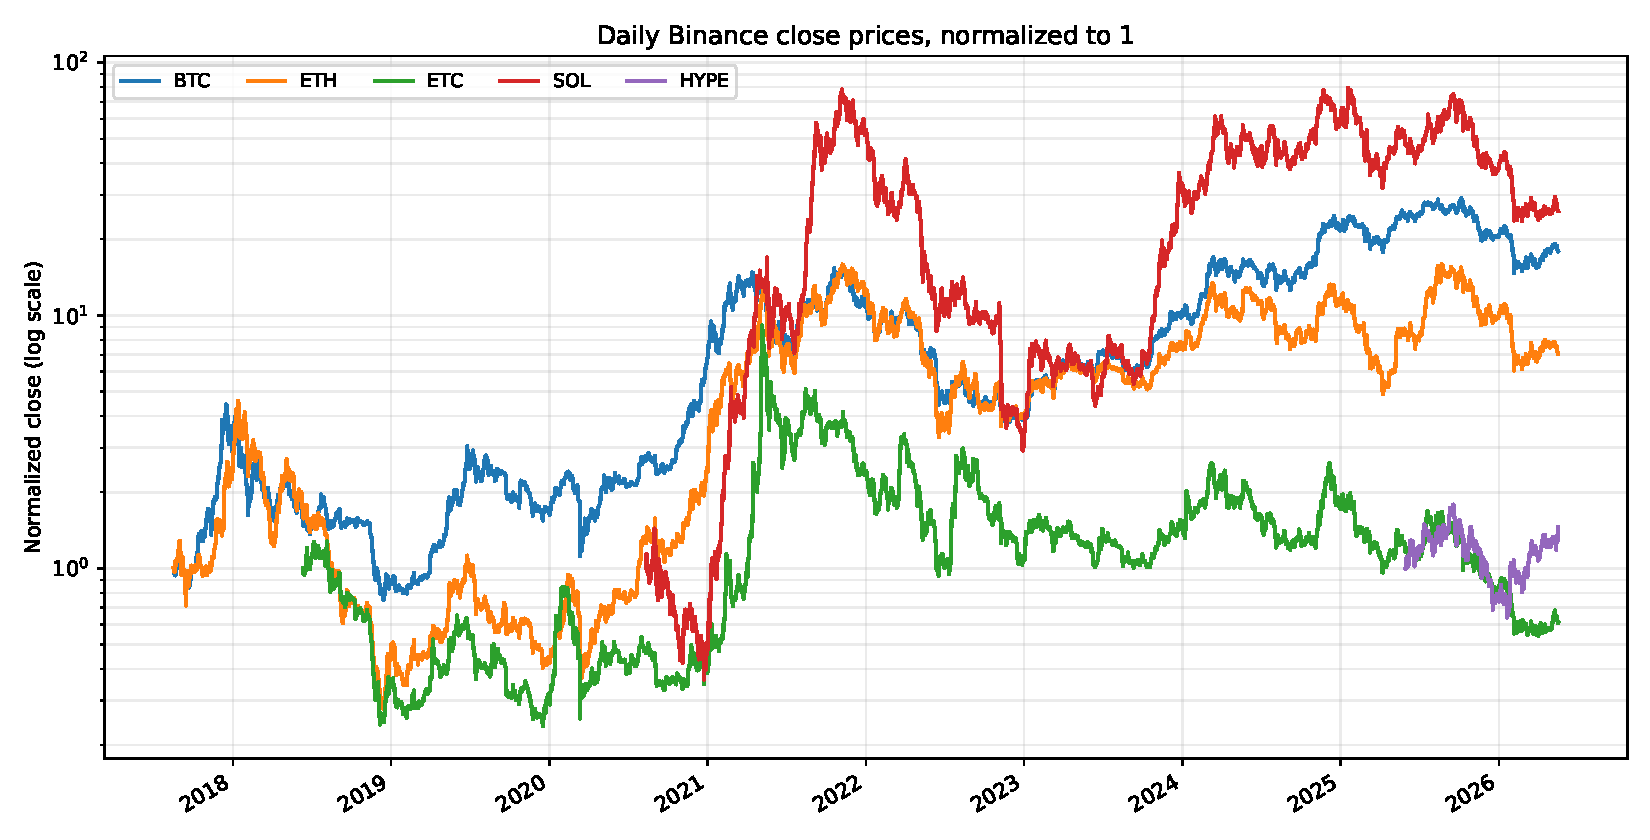
\includegraphics[width=0.98\textwidth]{regime_chapter_figs/fig01_normalized_prices.pdf}
\caption{Downloaded daily close prices, normalized to 1 at each asset's first available row. A log scale is used because crypto prices can move by orders of magnitude.}
\end{figure}

\begin{table}[H]
\centering
\scriptsize
\setlength{\tabcolsep}{3pt}
\resizebox{\textwidth}{!}{%
\begin{tabular}{@{}llccrrcrcccr@{}}
\toprule
Asset & Source & Raw start & Raw end & Raw rows & $\tau$ & SDFC candidate & SDFC $t$ & Max SADF & Max CSW & Max SMT & Runs \\
\midrule
%%SUMMARY_ROWS%%
\bottomrule
\end{tabular}}
\caption{Daily Binance data and headline diagnostic results. $\tau$ is the minimum daily window length used in recursive tests. Runs count retrospective consensus alert runs, where at least two diagnostic families were simultaneously in their research-alert region.}
\end{table}

\begin{table}[H]
\centering
\small
\begin{tabular}{@{}lp{0.60\textwidth}@{}}
\toprule
Parameter & Value \\
\midrule
%%PARAMETER_ROWS%%
\bottomrule
\end{tabular}
\caption{Backtest and diagnostic parameters used by the generated report.}
\end{table}

\section{Diagnostic Families}

The table below maps each statistic in this report to the source material it is based on, so readers can connect the empirical output back to the original definitions.

\begin{table}[H]
\centering
\small
\begin{tabular}{@{}lll@{}}
\toprule
Report statistic & Source & Fidelity \\
\midrule
BDE-inspired CUSUM & AFML \S17.3.1 (Brown-Durbin-Evans 1975) & inspired, online variant \\
Two-sided CSW excess & AFML \S17.3.2 (Chu-Stinchcombe-White 1996) & two-sided heuristic \\
SDFC & AFML \S17.4.1 (Chow-type Dickey-Fuller) & faithful, zero-lag \\
SADF & AFML \S17.4.2 (Phillips-Wu-Yu 2011) & faithful, zero-lag \\
QADF / CADF & AFML \S17.4.2.4--17.4.2.5 & faithful, zero-lag \\
SMT score & AFML \S17.4.3 (SM-Exp/Power/Poly1/Poly2) & all four forms, one $\varphi$ \\
HMM regime filter & Hamilton (1989); Cartea et al.\ Ch.~12 & walk-forward, filtered \\
\bottomrule
\end{tabular}
\caption{Where each diagnostic comes from and how closely it follows the source definition.}
\end{table}

\subsection{CUSUM Tests}

CUSUM means cumulative sum. The BDE-inspired series in this report is a recursive one-step forecast-error CUSUM from a simple log-price trend model. At each close $t$ the trend model is refitted on all data before $t$, and the standardized forecast error
\[
    \hat\omega_t = \frac{y_t - \hat\alpha_{t-1} - \hat\beta_{t-1} t}{\hat\sigma_{t-1}\sqrt{1 + h_t}},
\]
where $h_t$ is the regression leverage of the new point, is accumulated into a scaled running sum. It is \textbf{not} a formal Brown-Durbin-Evans boundary test: residuals are normalized online with shifted expanding statistics so a value at close $t$ uses only information available through $t$.

The Chu-Stinchcombe-White statistic asks whether log price has moved too far from an earlier reference level relative to realized volatility:
\[
    S_{n,t} = \frac{y_t-y_n}{\hat\sigma_t\sqrt{t-n}},
    \qquad
    \hat\sigma_t^2 = \frac{1}{t-1}\sum_{i=2}^t (\Delta y_i)^2.
\]
The report applies the level-departure statistic symmetrically to bubbles and crashes. Because of that absolute-value transformation, the displayed CSW excess should be read as a two-sided heuristic rather than the original one-sided 5\% test.

\subsection{ADF-Style Tests}

SDFC scans for a single full-sample unknown break into an explosive alternative. It is not traded here because choosing the break date from the full sample would use future data. SADF, QADF, and CADF scan repeated backward windows ending at each date. The implementation uses the zero-lag ADF form for readability and speed:
\[
    \Delta y_t = \alpha + \beta y_{t-1} + \varepsilon_t.
\]
For formal interpretation, the report now adds cached finite-sample random-walk simulations for SADF/QADF/CADF critical values. The full-sample top 5\% plot flags remain research visualizations, not p-values.

\subsection{SMT-Style Trend Tests}

The sub/super-martingale score evaluates the four trend specifications from the source text: an exponential trend on log price (SM-Exp), a power trend of log price on log time (SM-Power), and quadratic trends on normalized raw price (SM-Poly1) and log price (SM-Poly2). For each specification the trend coefficient $\hat\beta_{t_0,t}$ is estimated on backward windows and the penalized absolute t-statistic is aggregated as
\[
    \mathrm{SMT}_t = \sup_{t_0 \in [1, t-\tau]}
    \left\{ \frac{\left|\hat\beta_{t_0,t}\right|}{\hat\sigma_{\beta_{t_0,t}}\,(t - t_0)^{\varphi}} \right\},
    \qquad \varphi = 0.5,
\]
where the penalty $(t-t_0)^{\varphi}$ prevents long windows from dominating through mechanically large t-values. High values flag unusually strong trend-like growth or collapse. They are useful features, but the reported score is a compact heuristic rather than a complete production SMT battery across many $\varphi$ values.

\subsection{Hidden Markov Regime Model}

In addition to the structural-break statistics, the report fits a Gaussian hidden Markov model (HMM) on two causal daily features: the one-day log return and a trailing multi-day log momentum. The HMM is a different kind of regime tool: instead of testing for a break against a reference model, it assumes the market switches between a small number of latent states $s_t$ following a Markov chain with transition matrix $A$, and that the observed feature vector is drawn from a state-specific Gaussian,
\[
    x_t \mid s_t = k \sim \mathcal{N}(\mu_k, \Sigma_k),
    \qquad
    \Pr[s_t = k \mid x_{1:t}] \propto
    \left( \textstyle\sum_j \Pr[s_{t-1} = j \mid x_{1:t-1}]\, A_{jk} \right) \mathcal{N}(x_t; \mu_k, \Sigma_k).
\]
The right-hand recursion is the \emph{filtered} state probability: it conditions only on observations up to $t$. This latent-state view goes back to Markov-switching models in econometrics and connects to the Markov-chain regime models used for order-flow states in the algorithmic-trading literature.

The implementation is designed so that no forward-looking information can reach the trading signal:
\begin{itemize}
    \item Parameters are re-estimated walk-forward on an expanding window at fixed refit dates; the model used at close $t$ was fitted only on data before its refit date, which is at or before $t$.
    \item The regime at close $t$ is the argmax of \emph{filtered} state probabilities from a causal forward pass over observations up to $t$. Smoothed (forward-backward) probabilities are never used out of sample, because smoothing conditions on future observations.
    \item The mapping from state index to bullish/non-bullish is computed from the training window only, by the state-weighted mean of same-window daily returns. If no state has a positive mean return, the signal stays flat.
    \item Like every other strategy in this report, the position is shifted by one day before it trades.
\end{itemize}
Assets with less history than the minimum training window (currently HYPE) remain flat and report an inactive HMM. The EM fit uses deterministic quantile-based initialization, so results are exactly reproducible without random seeds.

\section{Formal Inference Versus Research Features}

\begin{table}[H]
\centering
\scriptsize
\setlength{\tabcolsep}{4pt}
\resizebox{\textwidth}{!}{%
\begin{tabular}{@{}llll@{}}
\toprule
Statistic & Threshold type & Formal p-value? & Online? \\
\midrule
%%INFERENCE_ROWS%%
\bottomrule
\end{tabular}}
\caption{Interpretation labels for the report's diagnostics and strategy conversions.}
\end{table}

\section{How to Read the Plots}

Each asset figure has six panels: price, BDE-inspired recursive CUSUM, two-sided CSW excess, ADF-family statistics, SMT-style trend score, and the filtered HMM regime state. Orange shading marks \textbf{retrospective consensus alert periods}: at least two diagnostic families were in their full-sample top-alert region or exceeded the fixed CSW boundary. This shading is useful for visual structure clustering, but it is not an online trading signal. In the HMM panel, green shading marks the days on which the filtered bull state was active; unlike the orange shading, this \emph{is} the online strategy state.

The online strategy signals are separate. BDE, SADF, QADF, CADF, and SMT strategy events use prior expanding thresholds only. CSW strategy events use the current positive excess because the statistic already embeds its reference boundary. The HMM strategy holds a long position exactly while the filtered bull state is active. The filtered HMM state per day is also stored in each asset's diagnostics CSV.

\section{Results by Asset}

%%ASSET_SECTIONS%%

\section{Consensus Alert Periods}

The table below lists the first few retrospective periods in which at least two diagnostic families were active. Short alert runs are common because the tests are sensitive to local trend acceleration and volatility normalization.

\begin{longtable}{@{}llll@{}}
\caption{First listed retrospective consensus alert periods. Period length is counted in calendar days between the first and last daily alert observation. For assets with many daily runs, the table shows the first eight runs.}\\
\toprule
Asset & Start & End & Days \\
\midrule
\endfirsthead
\toprule
Asset & Start & End & Days \\
\midrule
\endhead
%%RUN_ROWS%%
\bottomrule
\end{longtable}

\begin{figure}[H]
\centering
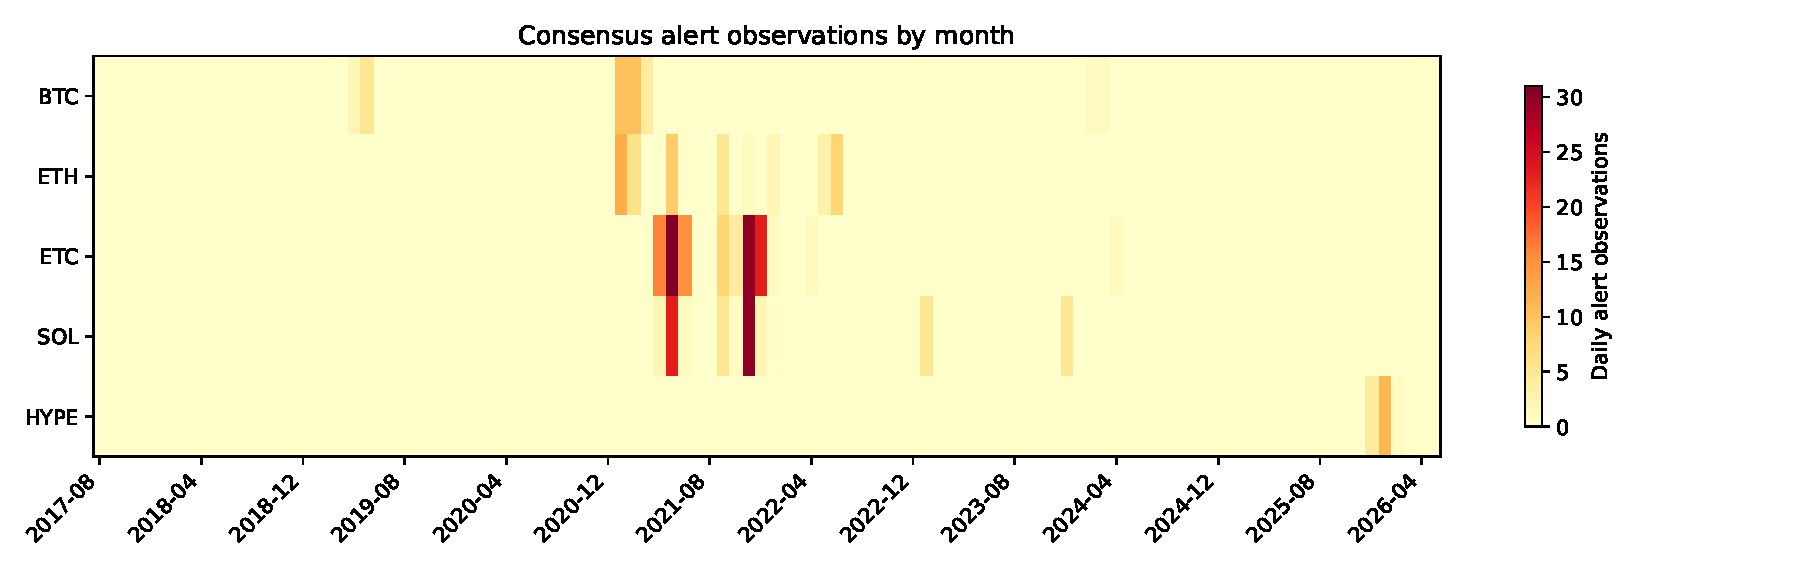
\includegraphics[width=0.98\textwidth]{regime_chapter_figs/fig02_alert_heatmap.pdf}
\caption{Retrospective consensus alert observations by month.}
\end{figure}

\section{Finite-Sample Calibration and Sensitivity}

The table below compares each asset's observed ADF-family maxima with cached random-walk finite-sample critical values. These simulations give a more defensible reference than the internal top 5\% visual flags, although they still inherit the simplified zero-lag ADF specification.

\begin{table}[H]
\centering
\scriptsize
\setlength{\tabcolsep}{3pt}
\resizebox{\textwidth}{!}{%
\begin{tabular}{@{}lrrrrrrrrrrr@{}}
\toprule
Asset & Sims & $\tau$ & SADF 95\% & Max SADF & SADF hits & QADF 95\% & Max QADF & QADF hits & CADF 95\% & Max CADF & CADF hits \\
\midrule
%%CRITICAL_ROWS%%
\bottomrule
\end{tabular}}
\caption{Simulated finite-sample critical values under random-walk null paths with matching sample length and $\tau$. Hits count daily observations above the 95\% simulated max-statistic threshold.}
\end{table}

\begin{longtable}{@{}lrrcrlr@{}}
\caption{Sensitivity of selected results to the minimum-window fraction. ADF-family windows vary; BDE, CSW, SMT, and HMM inputs are held at their main-run definitions.}\\
\toprule
Asset & $\tau$ rule & $\tau$ & Max SADF date & Runs & Best structure signal & Final \\
\midrule
\endfirsthead
\toprule
Asset & $\tau$ rule & $\tau$ & Max SADF date & Runs & Best structure signal & Final \\
\midrule
\endhead
%%TAU_SENSITIVITY_ROWS%%
\bottomrule
\end{longtable}

\section{Long/Flat Backtests}

The diagnostics above are research features, not trading rules. Still, it is useful to ask what a simple long-or-cash conversion would have done.

\subsection{Backtest Rule}

\begin{enumerate}
    \item At each daily close $t$, compute diagnostics using data through $t$ only.
    \item Convert each eligible indicator into an online alert using prior expanding thresholds, except CSW, whose positive excess is already boundary-based.
    \item Require the trailing momentum gate to be positive.
    \item An alert computed at close $t$ sets exposure for the close $t$ to close $t+1$ return, assuming execution at or immediately after close $t$.
    \item Keep the position long for the holding window after a valid alert, then move back out unless a new alert refreshes the holding window. The HMM strategy is the exception: it uses no momentum gate and no holding window, and instead stays long exactly while the filtered bull state is active.
    \item Charge transaction costs whenever exposure changes. Buy-and-hold is charged one entry cost for consistency.
\end{enumerate}

This is still an in-sample comparison. The best final PnL is an indicative ranking of which simple signal conversion looked promising on this sample, not evidence of a deployable strategy.

\begin{table}[H]
\centering
\scriptsize
\setlength{\tabcolsep}{4pt}
\resizebox{\textwidth}{!}{%
\begin{tabular}{@{}llrrlrrr@{}}
\toprule
Asset & Best structure signal & Best signal final & Buy-and-hold final & Best including buy-and-hold & Max DD & Exposure & Trades \\
\midrule
%%STRATEGY_BEST_ROWS%%
\bottomrule
\end{tabular}}
\caption{Best long/flat structure-break strategy by final equity multiple. Best structure signal excludes buy-and-hold; best including buy-and-hold includes it. Max DD, exposure, and trades refer to the best structure signal.}
\end{table}

\begin{figure}[H]
\centering
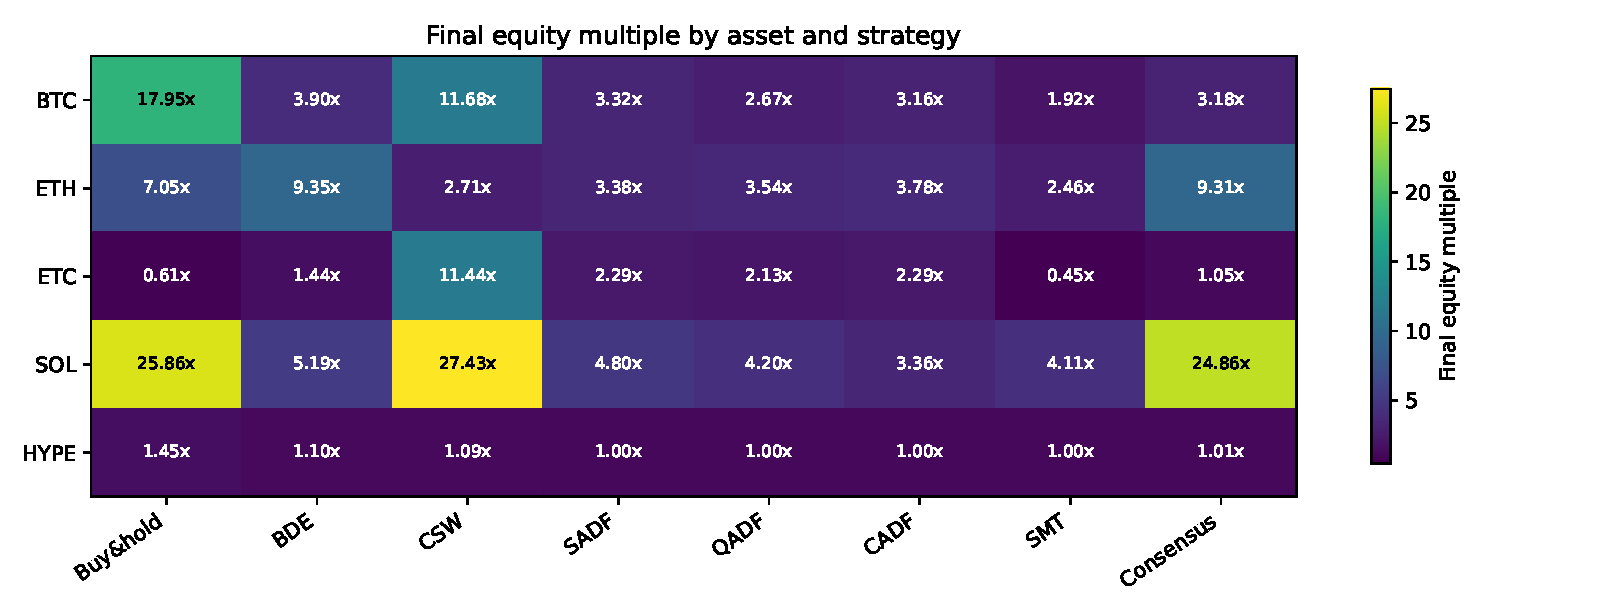
\includegraphics[width=0.98\textwidth]{regime_chapter_figs/fig_strategy_final_multiple_heatmap.pdf}
\caption{Final equity multiple by asset and strategy. Values are in-sample and normalized to 1 at each asset's first available observation.}
\end{figure}

\subsection{PnL Curves}

\begin{figure}[H]
\centering
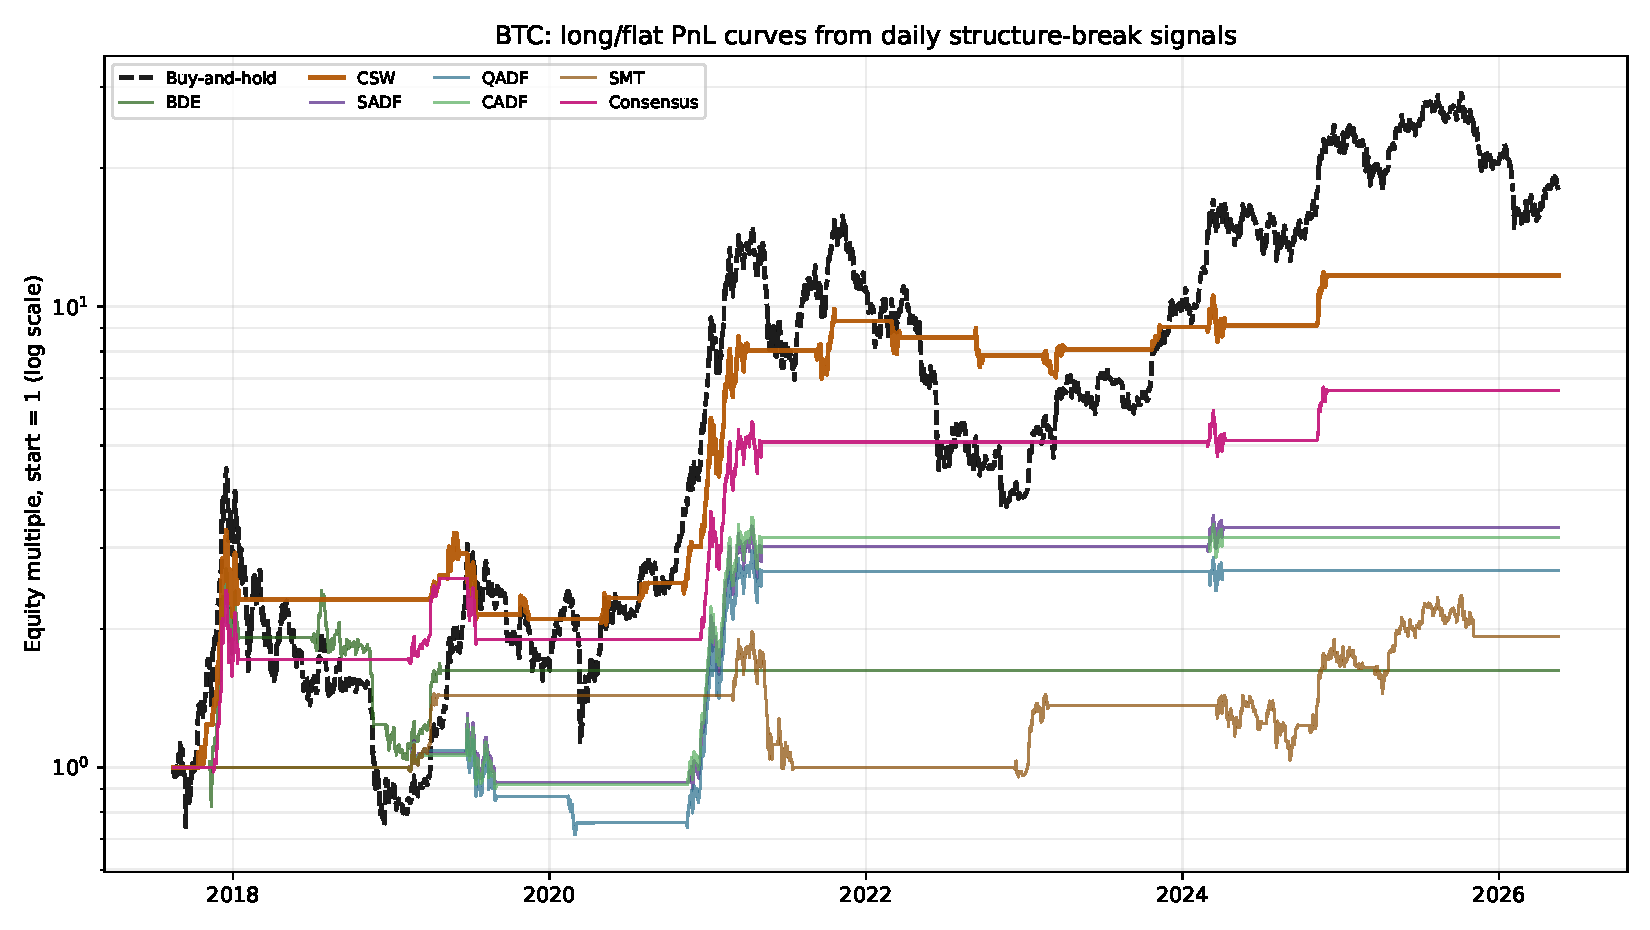
\includegraphics[width=0.98\textwidth]{regime_chapter_figs/fig_strategy_pnl_BTC.pdf}
\caption{BTC long/flat strategy PnL curves.}
\end{figure}

\begin{figure}[H]
\centering
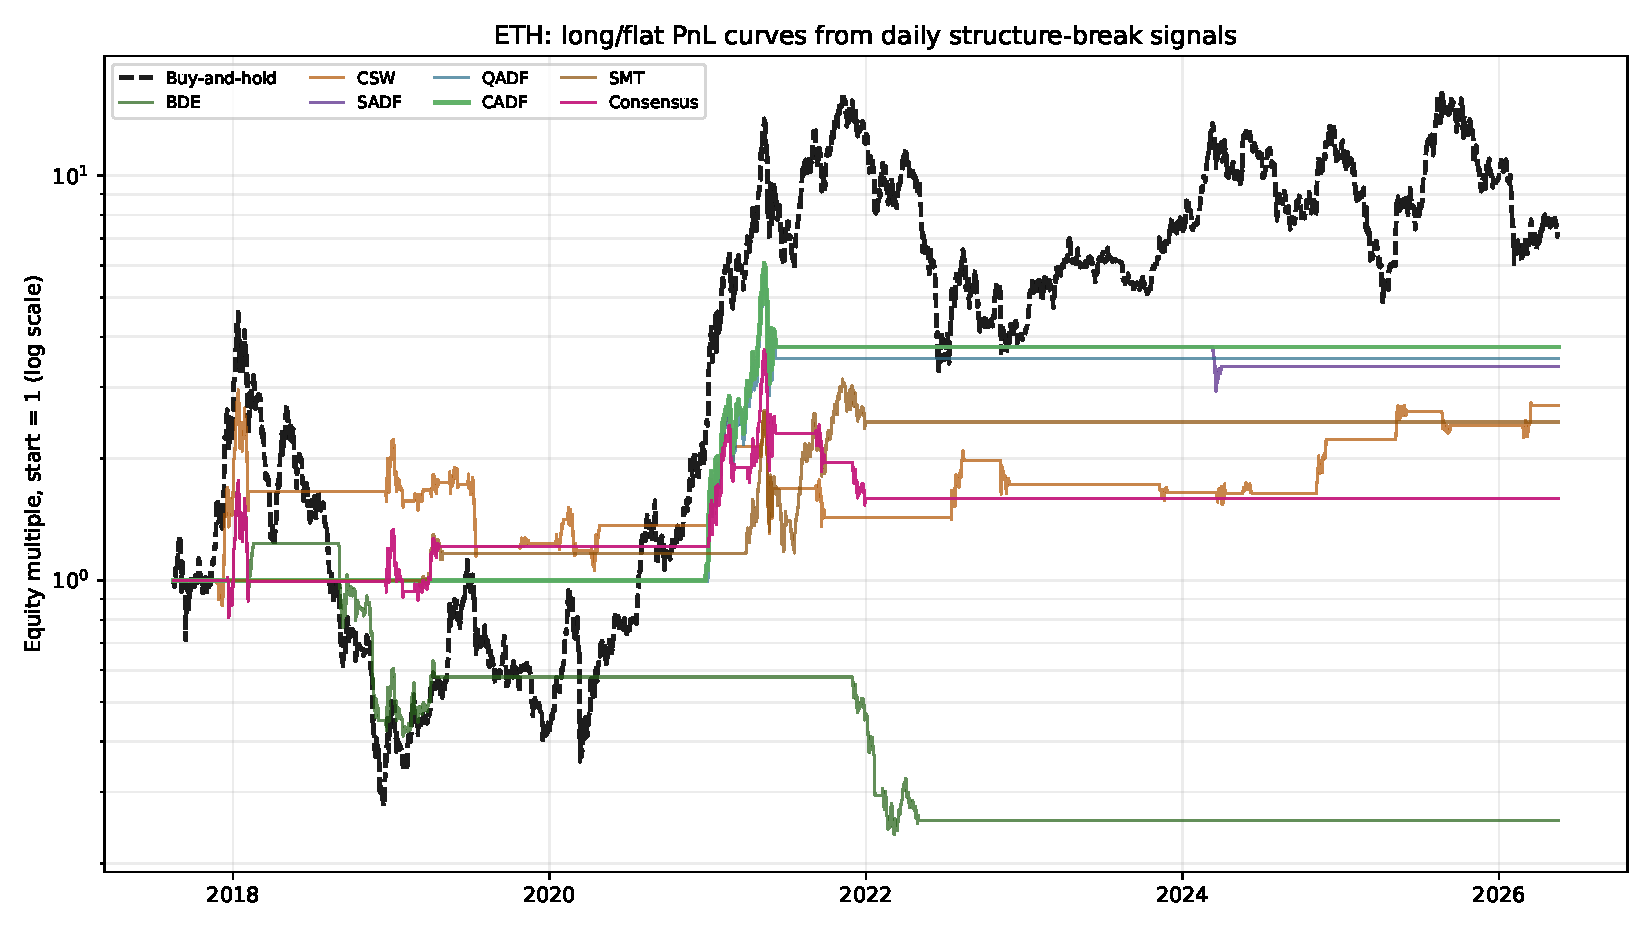
\includegraphics[width=0.98\textwidth]{regime_chapter_figs/fig_strategy_pnl_ETH.pdf}
\caption{ETH long/flat strategy PnL curves.}
\end{figure}

\begin{figure}[H]
\centering
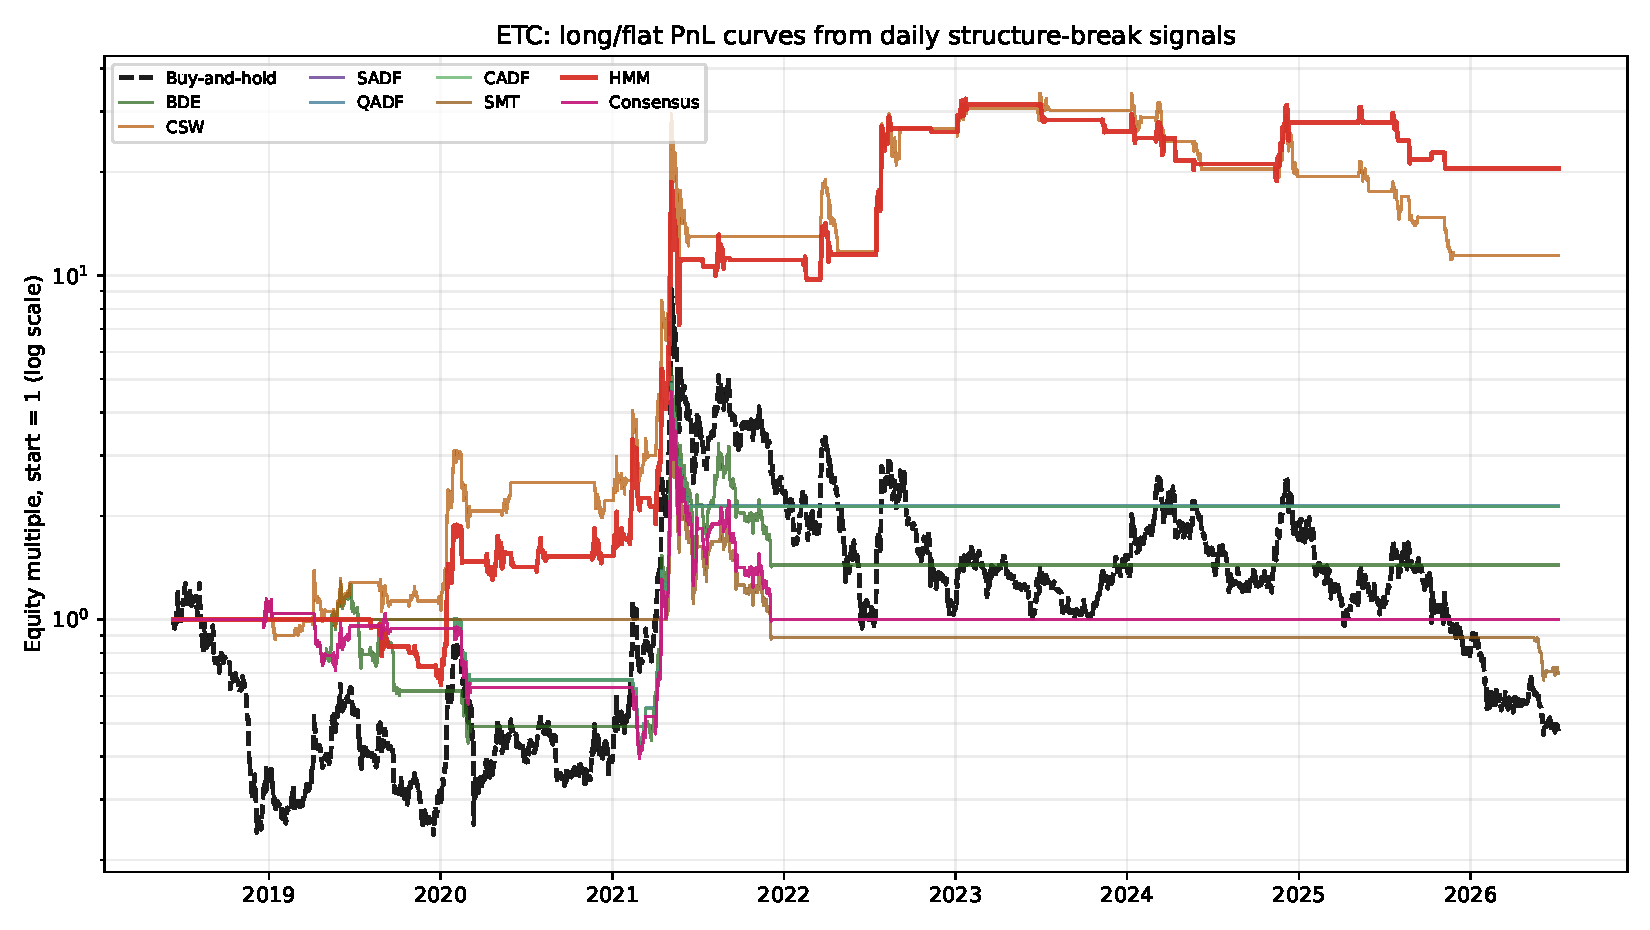
\includegraphics[width=0.98\textwidth]{regime_chapter_figs/fig_strategy_pnl_ETC.pdf}
\caption{ETC long/flat strategy PnL curves.}
\end{figure}

\begin{figure}[H]
\centering
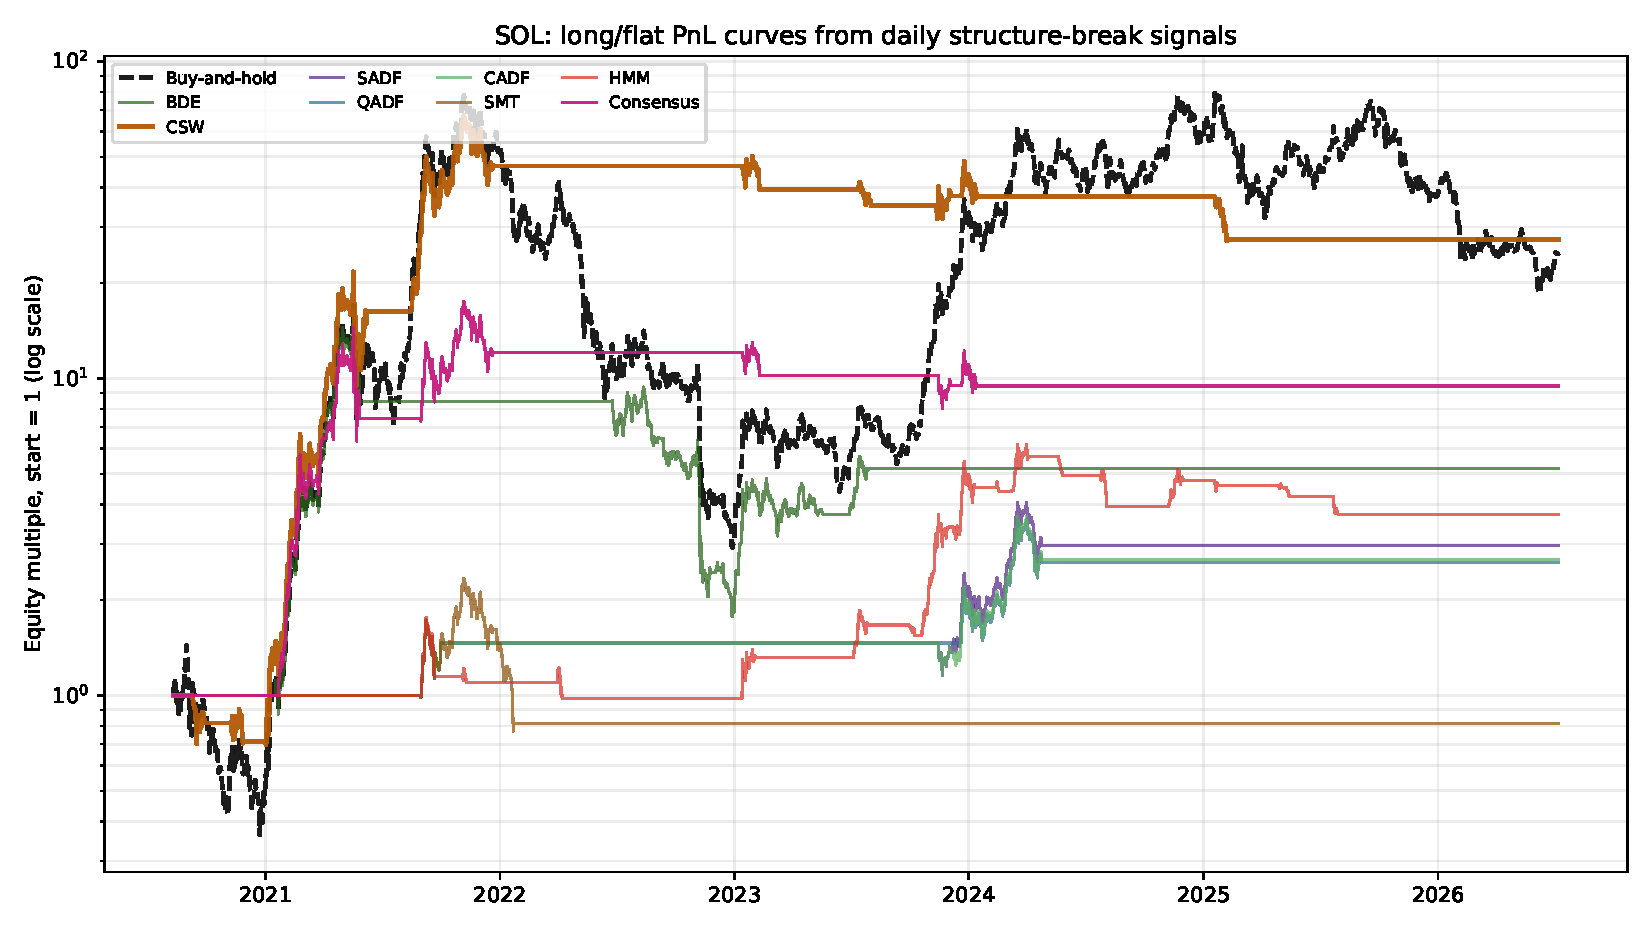
\includegraphics[width=0.98\textwidth]{regime_chapter_figs/fig_strategy_pnl_SOL.pdf}
\caption{SOL long/flat strategy PnL curves.}
\end{figure}

\begin{figure}[H]
\centering
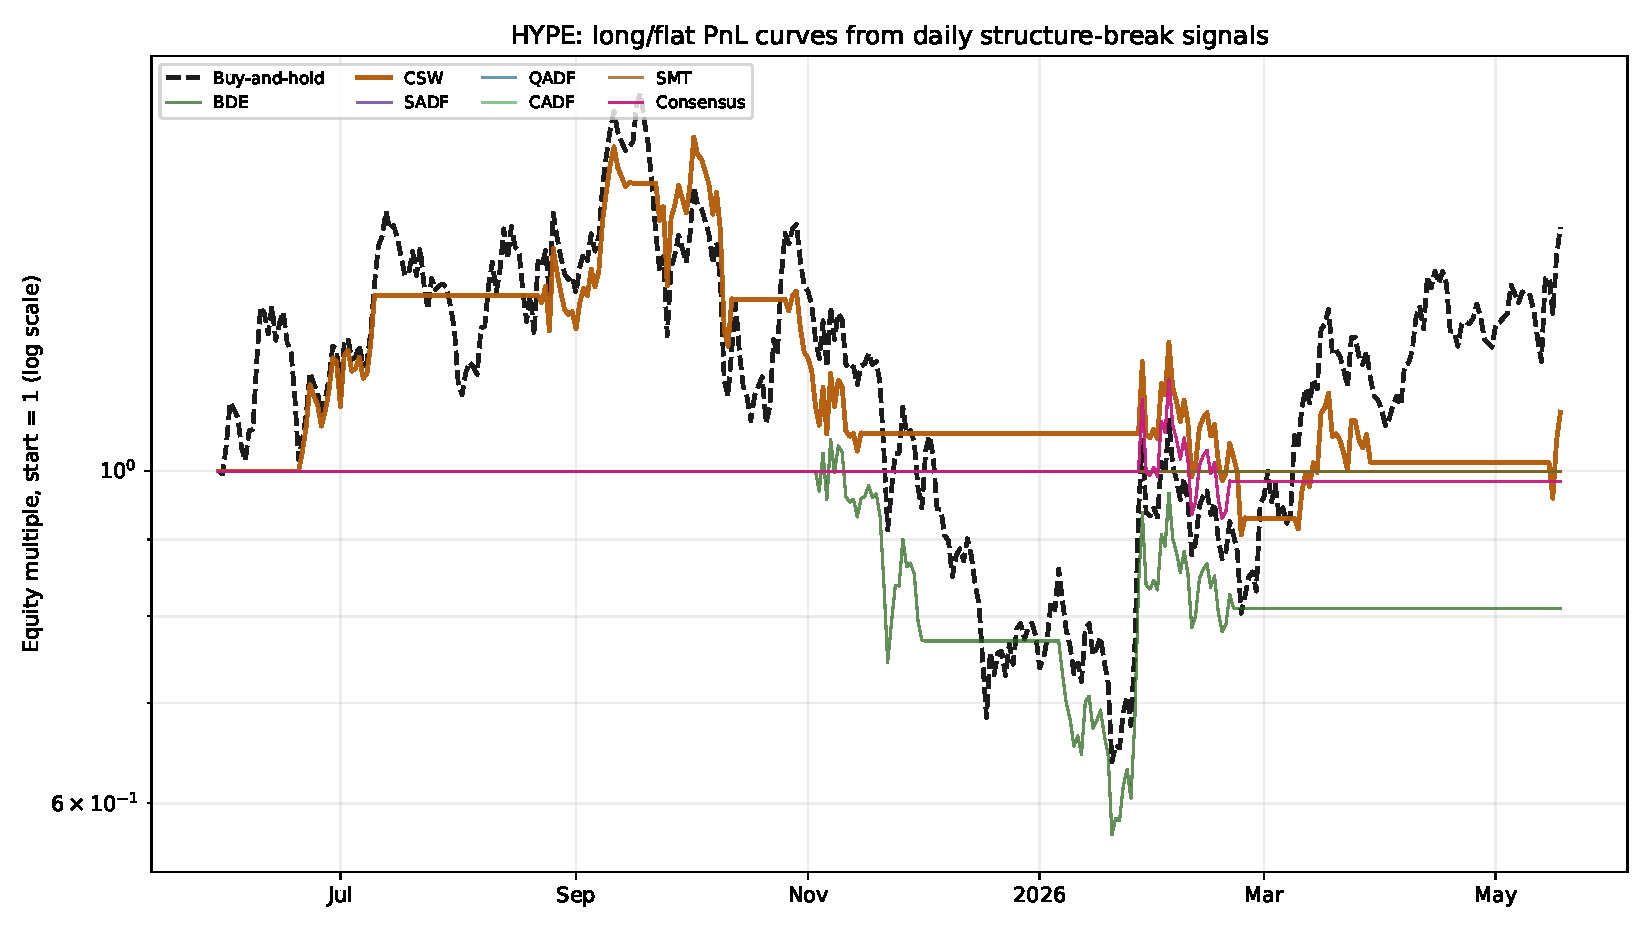
\includegraphics[width=0.98\textwidth]{regime_chapter_figs/fig_strategy_pnl_HYPE.pdf}
\caption{HYPE long/flat strategy PnL curves. HYPE uses Binance USD-M futures price data; returns exclude funding and futures-specific carry.}
\end{figure}

\subsection{Full Strategy Table}

\begin{longtable}{@{}llrrrrrrr@{}}
\caption{Simple long/flat strategy performance. Final multiple is the ending equity multiple from 1. CAGR is annualized over each asset's available sample. Sharpe uses daily returns and 365-day annualization. Because Sharpe is computed from arithmetic daily means, a volatile asset can show a positive Sharpe while its compounded return is negative (volatility drag); ETC buy-and-hold is an example.}\\
\toprule
Asset & Strategy & Final & Total return & CAGR & Max DD & Sharpe & Exposure & Trades \\
\midrule
\endfirsthead
\toprule
Asset & Strategy & Final & Total return & CAGR & Max DD & Sharpe & Exposure & Trades \\
\midrule
\endhead
%%STRATEGY_DETAIL_ROWS%%
\bottomrule
\end{longtable}

\subsection{Walk-Forward and Multiple-Testing Checks}

The walk-forward check selects the best structure signal on an expanding training window and evaluates only the next out-of-sample block. This does not prove profitability, but it reduces the most obvious winner-picking bias in the in-sample table. In the selected-signal path, repeated selections are compressed, so ``CSW x6'' means CSW was chosen for six consecutive blocks.

\begin{table}[H]
\centering
\scriptsize
\setlength{\tabcolsep}{4pt}
\resizebox{\textwidth}{!}{%
\begin{tabular}{@{}lrrlrrr@{}}
\toprule
Asset & Blocks & OOS days & Selected signal path & OOS final & OOS Sharpe & OOS Max DD \\
\midrule
%%WALK_FORWARD_ROWS%%
\bottomrule
\end{tabular}}
\caption{Expanding-window walk-forward validation of signal selection. HYPE has too little history for the default train/test split and may show no blocks.}
\end{table}

\begin{table}[H]
\centering
\scriptsize
\setlength{\tabcolsep}{4pt}
\resizebox{\textwidth}{!}{%
\begin{tabular}{@{}lrlrrrl@{}}
\toprule
Asset & Bootstrap sims & Best signal & Best final & Final 5--95\% CI & Sharpe 5--95\% CI & Reality-check $p$ \\
\midrule
%%BOOTSTRAP_ROWS%%
\bottomrule
\end{tabular}}
\caption{Block-bootstrap uncertainty for the best in-sample structure signal and a simple centered bootstrap reality-check p-value for best excess mean return versus buy-and-hold.}
\end{table}

The reality-check p-value estimates how often a resampled, mean-centered version of the signal family would produce a best mean daily excess return over buy-and-hold at least as large as the one observed, after accounting for the fact that the best of several signals was selected. Values near 1 mean the observed outperformance is entirely consistent with luck; only small values (for example below 0.05) would count as evidence of skill. Readers should check the table rather than assume the headline equity multiples imply significance.

\section{Interpretation}

Methodologically, SADF is a strong default diagnostic for repeated explosive episodes because it does not require the analyst to know the number or timing of regime switches. Empirically, in this particular in-sample long/flat conversion, the winning signal can differ by asset and must be treated as selected after looking at many alternatives.

The most important traps are multiple testing, listing-history differences, simplified zero-lag ADF regressions, and price-only data. HYPE is especially limited because it uses futures price klines without funding-rate adjustment. The HMM adds a complementary latent-state view, but its in-sample equity multiples share the same selection caveats, and its output is sensitive to the number of states and the refit schedule. Regime-change diagnostics are best read as feature-engineering tools, not as a recipe for direct trading.

\section{Minimal Reproducibility Sketch}

\begin{lstlisting}[language=Python]
# online execution convention used in the backtest
event_t = signal_at_close_t
position = event_t.rolling(hold_days).max().shift(1)
strategy_return_t = position_t * close.pct_change_t - costs_t

# HMM variant: no hold window, position tracks the filtered bull state
position_hmm = (filtered_state_at_close_t == bull_state).shift(1)
\end{lstlisting}

\section{Reproduce}

\begin{lstlisting}[language=bash]
python3 scripts/generate_daily_regime_chapter.py --use-cache
pdflatex -interaction=nonstopmode regime_detection_crypto_report.tex
pdflatex -interaction=nonstopmode regime_detection_crypto_report.tex
\end{lstlisting}

The generator writes daily diagnostics, strategy PnL CSVs, cached calibration files, strict JSON metadata, all figures, and this TeX report. The rendered PDF is then produced by \texttt{pdflatex}.

\section{References}

\begin{itemize}
    \item Marcos L\'opez de Prado, \emph{Advances in Financial Machine Learning}, Wiley, 2018, structural-break methods (Chapter 17).
    \item \'Alvaro Cartea, Sebastian Jaimungal, and Jos\'e Penalva, \emph{Algorithmic and High-Frequency Trading}, Cambridge University Press, 2015, Markov-chain regime models for order flow (Chapter 12), motivating the latent-regime view used by the HMM filter.
    \item R.~L.~Brown, J.~Durbin, and J.~M.~Evans, ``Techniques for testing the constancy of regression relationships over time,'' \emph{Journal of the Royal Statistical Society B}, 37(2), 1975.
    \item C.-S.~J.~Chu, M.~Stinchcombe, and H.~White, ``Monitoring structural change,'' \emph{Econometrica}, 64(5), 1996; and U.~Homm and J.~Breitung, ``Testing for speculative bubbles in stock markets,'' \emph{Journal of Financial Econometrics}, 10(1), 2012.
    \item G.~C.~Chow, ``Tests of equality between sets of coefficients in two linear regressions,'' \emph{Econometrica}, 28(3), 1960.
    \item P.~C.~B.~Phillips, Y.~Wu, and J.~Yu, ``Explosive behavior in the 1990s Nasdaq: When did exuberance escalate asset values?'' \emph{International Economic Review}, 52(1), 2011.
    \item J.~D.~Hamilton, ``A new approach to the economic analysis of nonstationary time series and the business cycle,'' \emph{Econometrica}, 57(2), 1989, the canonical Markov-switching regime model.
    \item Binance API daily kline endpoints for BTCUSDT, ETHUSDT, ETCUSDT, SOLUSDT spot, and HYPEUSDT USD-M futures fallback.
    \item Local reproduction script: \texttt{scripts/generate\_daily\_regime\_chapter.py}.
\end{itemize}

\end{document}
